\documentclass[11pt,a4paper]{report}
\usepackage[textwidth=37em,vmargin=30mm]{geometry}
\usepackage{calc,xunicode,amsmath,amssymb,paralist,enumitem,tabu,booktabs,datetime2,xeCJK,xeCJKfntef,listings}
\usepackage{tocloft,fancyhdr,tcolorbox,xcolor,graphicx,eso-pic,xltxtra,xelatexemoji}

\newcommand{\envyear}[0]{2025}
\newcommand{\envdatestr}[0]{2025-10-31}
\newcommand{\envfinaldir}[0]{webdb/2025/20251031/final}

\usepackage[hidelinks]{hyperref}
\hypersetup{
    colorlinks=false,
    pdfpagemode=FullScreen,
    pdftitle={Web Digest - \envdatestr}
}

\setlength{\cftbeforechapskip}{10pt}
\renewcommand{\cftchapfont}{\rmfamily\bfseries\large\raggedright}
\setlength{\cftbeforesecskip}{2pt}
\renewcommand{\cftsecfont}{\sffamily\small\raggedright}

\setdefaultleftmargin{2em}{2em}{1em}{1em}{1em}{1em}

\usepackage{xeCJK,xeCJKfntef}
\xeCJKsetup{PunctStyle=plain,RubberPunctSkip=false,CJKglue=\strut\hskip 0pt plus 0.1em minus 0.05em,CJKecglue=\strut\hskip 0.22em plus 0.2em}
\XeTeXlinebreaklocale "zh"
\XeTeXlinebreakskip = 0pt


\setmainfont{Brygada 1918}
\setromanfont{Brygada 1918}
\setsansfont{IBM Plex Sans}
\setmonofont{JetBrains Mono NL}
\setCJKmainfont{Noto Serif CJK SC}
\setCJKromanfont{Noto Serif CJK SC}
\setCJKsansfont{Noto Sans CJK SC}
\setCJKmonofont{Noto Sans CJK SC}

\setlength{\parindent}{0pt}
\setlength{\parskip}{8pt}
\linespread{1.15}

\lstset{
	basicstyle=\ttfamily\footnotesize,
	numbersep=5pt,
	backgroundcolor=\color{black!5},
	showspaces=false,
	showstringspaces=false,
	showtabs=false,
	tabsize=2,
	captionpos=b,
	breaklines=true,
	breakatwhitespace=true,
	breakautoindent=true,
	linewidth=\textwidth
}






\newcommand{\coverpic}[2]{
    % argv: itemurl, authorname
    Cover photo by #2~~(\href{#1}{#1})
}
\newcommand{\makeheader}[0]{
    \begin{titlepage}
        % \newgeometry{hmargin=15mm,tmargin=21mm,bmargin=12mm}
        \begin{center}
            
            \rmfamily\scshape
            \fontspec{BaskervilleF}
            \fontspec{Old Standard}
            \fontsize{59pt}{70pt}\selectfont
            WEB\hfill DIGEST
            
            \vfill
            % \vskip 30pt
            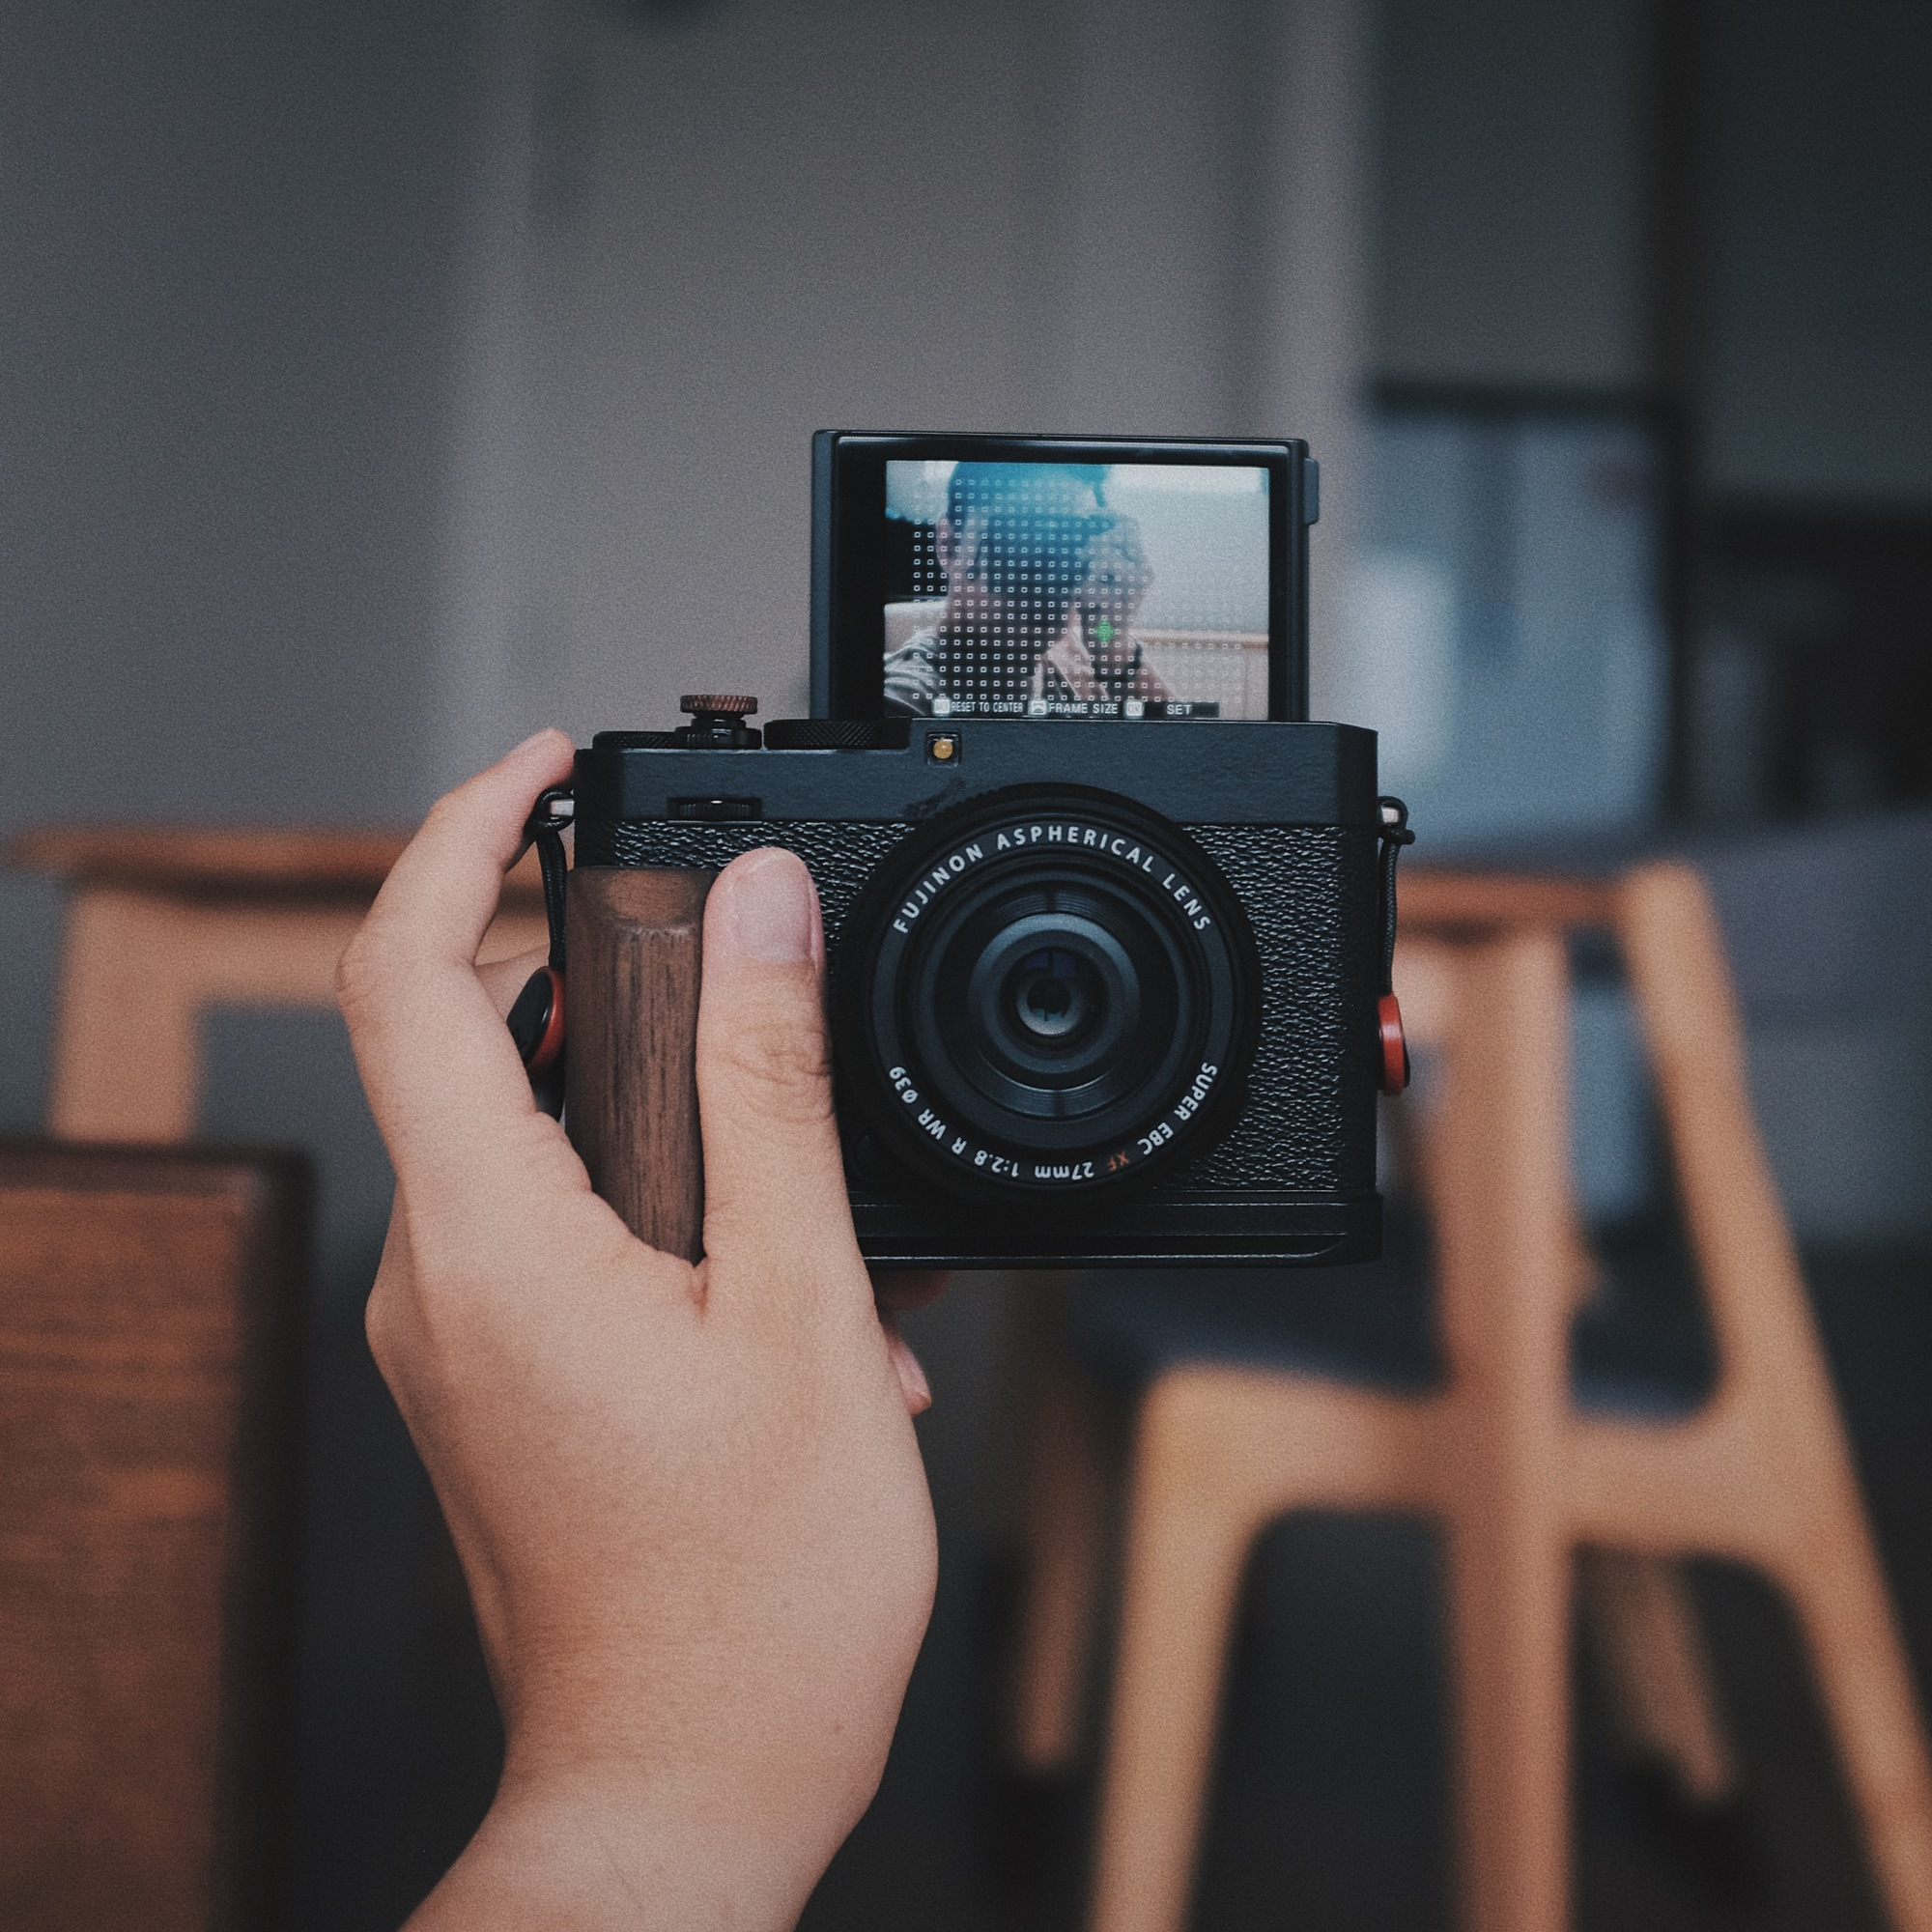
\includegraphics[width=\linewidth]{\envfinaldir/coverpic-prod.jpg}\par
            % \vskip 30pt
            \vfill

            \normalsize\rmfamily\scshape
            \copyright{} The Web Digest Project \hfill\large \envdatestr
        \end{center}
    \end{titlepage}
    % \restoregeometry
}
\newcommand{\simplehref}[1]{%
    \textcolor{blue!80!green}{\href{#1}{#1}}%
}
\renewcommand{\contentsname}{\center\Huge\sffamily\bfseries Contents\par\vskip 20pt}
\newcounter{ipartcounter}
\setcounter{ipartcounter}{0}
\newcommand{\ipart}[1]{
    % \vskip 20pt
    \clearpage
    \stepcounter{ipartcounter}
    \phantomsection
    \addcontentsline{toc}{chapter}{#1}
    % \begin{center}
    %     \Huge
    %     \sffamily\bfseries
    %     #1
    % \end{center}
    % \vskip 20pt plus 7pt
}
\newcounter{ichaptercounter}
\setcounter{ichaptercounter}{0}
\newcommand{\ichapter}[1]{
    % \vskip 20pt
    \clearpage
    \stepcounter{ichaptercounter}
    \phantomsection
    \addcontentsline{toc}{section}{\numberline{\arabic{ichaptercounter}}#1}
    \begin{center}
        \Huge
        \sffamily\bfseries
        #1
    \end{center}
    \vskip 20pt plus 7pt
}
\newcommand{\entrytitlefont}[1]{\subsection*{\raggedright\Large\sffamily\bfseries#1}}
\newcommand{\entryitemGeneric}[2]{
    % argv: title, url
    \parbox{\linewidth}{
        \entrytitlefont{#1}\par\vskip 5pt
        \footnotesize\ttfamily\mdseries
        \simplehref{#2}
    }\vskip 11pt plus 11pt minus 1pt
}
\newcommand{\entryitemGithub}[3]{
    % argv: title, url, desc
    \parbox{\linewidth}{
        \entrytitlefont{#1}\par\vskip 5pt
        \footnotesize\ttfamily\mdseries
        \simplehref{#2}\par\vskip 5pt
        \small\rmfamily\mdseries#3
    }\vskip 11pt plus 11pt minus 1pt
}
\newcommand{\entryitemAp}[3]{
    % argv: title, url, desc
    \parbox{\linewidth}{
        \entrytitlefont{#1}\par\vskip 5pt
        \footnotesize\ttfamily\mdseries
        \simplehref{#2}\par\vskip 5pt
        \small\rmfamily\mdseries#3
    }\vskip 11pt plus 11pt minus 1pt
}
\newcommand{\entryitemHackernews}[3]{
    % argv: title, hnurl, rawurl
    % \parbox{\linewidth}{
    %     \entrytitlefont{#1}\par\vskip 5pt
    %     \footnotesize\ttfamily\mdseries
    %     \simplehref{#3}\par
    %     \textcolor{black!50}{\href{#2}{#2}}
    % }\vskip 11pt plus 11pt minus 1pt
    \begin{minipage}{\linewidth}
            \entrytitlefont{#1}\par\vskip 5pt
            \footnotesize\ttfamily\mdseries
            \simplehref{#3}\par
            \textcolor{black!50}{\href{#2}{#2}}
    \end{minipage}\par\vskip 11pt plus 11pt minus 1pt
}







\begin{document}

\makeheader

\tableofcontents\clearpage




\ipart{Developers}
\ichapter{Hacker News}
\entryitemTwoLinks{A change of address led to our Wise accounts being shut down}{https://news.ycombinator.com/item?id=45766253}{https://shaun.nz/why-were-never-using-wise-again-a-cautionary-tale-from-a-business-burned/}

\entryitemTwoLinks{Denmark reportedly withdraws Chat Control proposal following controversy}{https://news.ycombinator.com/item?id=45765664}{https://therecord.media/demark-reportedly-withdraws-chat-control-proposal}

\entryitemTwoLinks{Taking money off the table}{https://news.ycombinator.com/item?id=45763769}{https://zachholman.com/posts/money-off-the-table}

\entryitemTwoLinks{I have released a 69.0MB version of Windows 7 x86}{https://news.ycombinator.com/item?id=45763076}{https://twitter.com/XenoPanther/status/1983477707968291075}

\entryitemTwoLinks{Some people can't see mental images}{https://news.ycombinator.com/item?id=45762837}{https://www.newyorker.com/magazine/2025/11/03/some-people-cant-see-mental-images-the-consequences-are-profound}

\entryitemTwoLinks{The ear does not do a Fourier transform}{https://news.ycombinator.com/item?id=45762259}{https://www.dissonances.blog/p/the-ear-does-not-do-a-fourier-transform}

\entryitemTwoLinks{Falling panel prices lead to global solar boom, except for the US}{https://news.ycombinator.com/item?id=45761902}{https://arstechnica.com/science/2025/10/theres-a-global-boom-in-solar-except-in-the-united-states/}

\entryitemTwoLinks{Qt Creator 18 Released}{https://news.ycombinator.com/item?id=45761789}{https://www.qt.io/blog/qt-creator-18-released}

\entryitemTwoLinks{Affinity Studio now free}{https://news.ycombinator.com/item?id=45761445}{https://www.affinity.studio/get-affinity}

\entryitemTwoLinks{PlanetScale Offering \$5 Databases}{https://news.ycombinator.com/item?id=45761027}{https://planetscale.com/blog/5-dollar-planetscale}

\entryitemTwoLinks{Free software scares normal people}{https://news.ycombinator.com/item?id=45760878}{https://danieldelaney.net/normal/}

\entryitemTwoLinks{Ventoy: Create bootable USB drive for ISO/WIM/IMG/VHD(x)/EFI Files}{https://news.ycombinator.com/item?id=45760340}{https://github.com/ventoy/Ventoy}

\entryitemTwoLinks{US declines to join more than 70 countries in signing UN cybercrime treaty}{https://news.ycombinator.com/item?id=45760328}{https://therecord.media/us-declines-signing-cybercrime-treaty?}

\entryitemTwoLinks{Show HN: I made a heatmap diff viewer for code reviews}{https://news.ycombinator.com/item?id=45760321}{https://0github.com}

\entryitemTwoLinks{The International Criminal Court wants to become independent of USA technology}{https://news.ycombinator.com/item?id=45759891}{https://www.heise.de/en/news/International-Criminal-Court-Kicks-Out-Microsoft-10964189.html}

\entryitemTwoLinks{Jujutsu at Google [video]}{https://news.ycombinator.com/item?id=45759572}{https://www.youtube.com/watch?v=v9Ob5yPpC0A}

\entryitemTwoLinks{Alphabet tops \$100B quarterly revenue for first time, cloud grows 34\%}{https://news.ycombinator.com/item?id=45758874}{https://www.cnbc.com/2025/10/29/alphabet-google-q3-earnings.html}

\entryitemTwoLinks{Show HN: In a single HTML file, an app to encourage my children to invest}{https://news.ycombinator.com/item?id=45758421}{https://roberdam.com/en/dinversiones.html}

\entryitemTwoLinks{Language models are injective and hence invertible}{https://news.ycombinator.com/item?id=45758093}{https://arxiv.org/abs/2510.15511}

\entryitemTwoLinks{Carlo Rovelli's radical perspective on reality}{https://news.ycombinator.com/item?id=45756445}{https://www.quantamagazine.org/carlo-rovellis-radical-perspective-on-reality-20251029/}\ichapter{Phoronix}
\entryitemGeneric{\hskip 0pt{}Rust 1.91 Promotes Windows On 64-bit ARM To Tier-1 Status}{https://www.phoronix.com/news/Rust-1.91-Released}

\entryitemGeneric{\hskip 0pt{}AMD ROCm 7.1 Released: Many Instinct MI350 Series Improvements, Better Performance}{https://www.phoronix.com/news/AMD-ROCm-7.1-Released}

\entryitemGeneric{\hskip 0pt{}AMD Strix Point Performance Continues Evolving Nicely With Ubuntu 25.10}{https://www.phoronix.com/review/amd-strix-point-ubuntu-2510}

\entryitemGeneric{\hskip 0pt{}LVFS + Fwupd Serve Up More Than 135 Million Firmware Downloads For Linux Users}{https://www.phoronix.com/news/LVFS-Fwupd-135-Million-Download}

\entryitemGeneric{\hskip 0pt{}New Linux Patch Expands The Range Of AMD Zen 6 CPU Models}{https://www.phoronix.com/news/Linux-Patch-More-Zen-6-Models}

\entryitemGeneric{\hskip 0pt{}Qt Creator 18 Released With Experimental Support For Development Containers}{https://www.phoronix.com/news/Qt-Creator-18-Released}

\entryitemGeneric{\hskip 0pt{}Ubuntu Announces Architecture Variants: Ubuntu 25.10 Gets x86\_64-v3 Packages}{https://www.phoronix.com/news/Ubuntu-Architecture-Variants}

\entryitemGeneric{\hskip 0pt{}AMD ROCm 7.1 Release Appears Imminent}{https://www.phoronix.com/news/AMD-ROCm-7.1-Imminent}

\entryitemGeneric{\hskip 0pt{}AMDGPU With Linux 6.19 Will Support Analog Video Connectors For Old GCN 1.0 GPUs}{https://www.phoronix.com/news/Linux-6.19-AMDGPU-Analog}


\ipart{Developers~~~~(zh-Hans)}
\ichapter{Solidot}
\entryitemGeneric{\hskip 0pt{}微软 XBox 掌机存在大量 Windows 系统问题}{https://www.solidot.org/story?sid=82676}

\entryitemGeneric{\hskip 0pt{}Pop!\_OS 24.04 LTS 将于 12 月推出}{https://www.solidot.org/story?sid=82675}

\entryitemGeneric{\hskip 0pt{}Grammarly 改名为 Superhuman}{https://www.solidot.org/story?sid=82674}

\entryitemGeneric{\hskip 0pt{}Tor Browser 15.0 释出}{https://www.solidot.org/story?sid=82673}

\entryitemGeneric{\hskip 0pt{}Fedora Linux 43 释出}{https://www.solidot.org/story?sid=82672}

\entryitemGeneric{\hskip 0pt{}英伟达成为第一家市值突破 5 万亿美元的公司}{https://www.solidot.org/story?sid=82671}

\entryitemGeneric{\hskip 0pt{}小鼠研究显示头发在 20 天内完全再生}{https://www.solidot.org/story?sid=82670}

\entryitemGeneric{\hskip 0pt{}矮星系发现巨大黑洞}{https://www.solidot.org/story?sid=82669}

\entryitemGeneric{\hskip 0pt{}澳大利亚警方开发大模型解码 Z 世代俚语和表情符号}{https://www.solidot.org/story?sid=82668}

\entryitemGeneric{\hskip 0pt{}外卖正在毁灭美国餐饮业}{https://www.solidot.org/story?sid=82667}

\entryitemGeneric{\hskip 0pt{}侧载究竟意味着什么?}{https://www.solidot.org/story?sid=82666}

\entryitemGeneric{\hskip 0pt{}接近九成 Windows 游戏能在 Linux 上运行}{https://www.solidot.org/story?sid=82665}

\entryitemGeneric{\hskip 0pt{}哈佛本科生六成成绩是 A}{https://www.solidot.org/story?sid=82664}

\entryitemGeneric{\hskip 0pt{}Python 基金会坚持 DEI 放弃美国政府的 150 万美元拨款}{https://www.solidot.org/story?sid=82663}

\entryitemGeneric{\hskip 0pt{}OpenAI 完成公司重组,微软持 27\% 股份和访问技术至 2032 年}{https://www.solidot.org/story?sid=82662}

\entryitemGeneric{\hskip 0pt{}社交圈扩大可能与社会极化相关}{https://www.solidot.org/story?sid=82661}

\entryitemGeneric{\hskip 0pt{}人类迁移的生物量超过所有陆地动物总和 40 倍}{https://www.solidot.org/story?sid=82660}

\entryitemGeneric{\hskip 0pt{}勒索软件的赎金支付比例创新低}{https://www.solidot.org/story?sid=82659}

\entryitemGeneric{\hskip 0pt{}GLP-1 减肥药降低了美国的肥胖率}{https://www.solidot.org/story?sid=82658}

\entryitemGeneric{\hskip 0pt{}阿尔巴尼亚的 AI 部长怀孕了}{https://www.solidot.org/story?sid=82657}\ichapter{V2EX}
\entryitemGeneric{\hskip 0pt{}[小米] 陈年旧事之小米是我成年之后第一个教训}{https://www.v2ex.com/t/1169572}

\entryitemGeneric{\hskip 0pt{}[NAS] 铁威马 F4-425Plus 和绿联 DXP4800 日常使用推荐那个啊}{https://www.v2ex.com/t/1169569}

\entryitemGeneric{\hskip 0pt{}[反馈] 急!我开启了 2FA,但是腾讯的身份验证器丢失了,也没有云端备份,如何重新绑定 2FA 呢?}{https://www.v2ex.com/t/1169567}

\entryitemGeneric{\hskip 0pt{}[问与答] 2080ti 22g 有什么效果还可以的 i2v 项目推荐}{https://www.v2ex.com/t/1169566}

\entryitemGeneric{\hskip 0pt{}[问与答] mac 有现成的"独立"剪切板工具吗? 与系统剪切板分开,互不打扰}{https://www.v2ex.com/t/1169565}

\entryitemGeneric{\hskip 0pt{}[宽带症候群] 实在没办法了,求助部分网站/软件无法访问的问题}{https://www.v2ex.com/t/1169564}

\entryitemGeneric{\hskip 0pt{}[职场话题] 广佛求职:是否只能拥抱外包?}{https://www.v2ex.com/t/1169563}

\entryitemGeneric{\hskip 0pt{}[问与答] 如果你有一次机会做一件对爱人不忠的事但可以完美免责,你会去做吗?}{https://www.v2ex.com/t/1169562}

\entryitemGeneric{\hskip 0pt{}[装修] 分享一下今年装修的经验}{https://www.v2ex.com/t/1169561}

\entryitemGeneric{\hskip 0pt{}[Apple] 告别最后一个 Lightning 接口设备}{https://www.v2ex.com/t/1169560}

\entryitemGeneric{\hskip 0pt{}[程序员] AI 相关问题讨论:低代码平台、智能体搭建工具和 Token 免费活动有哪些?}{https://www.v2ex.com/t/1169558}

\entryitemGeneric{\hskip 0pt{}[职场话题] 前同事分享的``背刺''前同事故事,离职后发现税前 6K 的工资被扣 600 块,发邮件给财务总监举报采购总监``渎职'',不是举报贪污}{https://www.v2ex.com/t/1169556}

\entryitemGeneric{\hskip 0pt{}[分享创造] Pomelli: Google 推出的免费生成网站营销海报的工具,效果惊艳}{https://www.v2ex.com/t/1169555}

\entryitemGeneric{\hskip 0pt{}[问与答] 天塌了, 在 Google Play 更新 GBoard 后,滑动输入时响应很慢}{https://www.v2ex.com/t/1169554}

\entryitemGeneric{\hskip 0pt{}[问与答] 煮八宝粥挑出来的冰糖积攒了一小袋了,要不要丢掉}{https://www.v2ex.com/t/1169553}

\entryitemGeneric{\hskip 0pt{}[投资] 记录自己对市场的理解与感悟}{https://www.v2ex.com/t/1169551}

\entryitemGeneric{\hskip 0pt{}[程序员] 为什么现在的开发者都不愿意写文档了?是真的没时间还是懒?}{https://www.v2ex.com/t/1169550}

\entryitemGeneric{\hskip 0pt{}[分享创造] 下班时间参考美图使用 Codex 搞了个拼图网站无需登录浏览器完成,目前 200+模板,可自定义、异形拼图、贴纸}{https://www.v2ex.com/t/1169549}

\entryitemGeneric{\hskip 0pt{}[程序员] 求推荐 AI 工具站开发模板}{https://www.v2ex.com/t/1169548}

\entryitemGeneric{\hskip 0pt{}[问与答] 问大家一个问题:如果你全力以赴的一件事,中途却发现结局与预想天差地别,你当时的心情是怎样?还会选择继续吗?}{https://www.v2ex.com/t/1169546}

\entryitemGeneric{\hskip 0pt{}[问与答] 从一个人的日常动作、面相、三言两语等能否大致判断此人的为人、性格特点等?}{https://www.v2ex.com/t/1169545}

\entryitemGeneric{\hskip 0pt{}[程序员] 今晚的生产环境事故是 B 站}{https://www.v2ex.com/t/1169544}

\entryitemGeneric{\hskip 0pt{}[问与答] 看到有人求赐名我也来求一个,不知道性别,姓张,预产期 12 月中旬 蛇宝}{https://www.v2ex.com/t/1169543}

\entryitemGeneric{\hskip 0pt{}[程序员] nextjs 16 正式版果然还只是个类似 beta 啊 要用的建议等到 16.1 或者 16.2 再碰}{https://www.v2ex.com/t/1169542}

\entryitemGeneric{\hskip 0pt{}[电影] 各位大神在电视上用什么播放器看本地电影}{https://www.v2ex.com/t/1169541}

\entryitemGeneric{\hskip 0pt{}[问与答] 碰到表单很多,表字段一多的需求开发就效率直线下降}{https://www.v2ex.com/t/1169539}

\entryitemGeneric{\hskip 0pt{}[Solana] HTTP 402 Payment Required 状态被启用,未来可能直接在浏览器端做支付了}{https://www.v2ex.com/t/1169537}

\entryitemGeneric{\hskip 0pt{}[推广] Claude pro 订阅代充值,欢迎 V 友咨询}{https://www.v2ex.com/t/1169536}

\entryitemGeneric{\hskip 0pt{}[生活] 聚餐时旁边的发小突然给我初恋打视频,我都懵了!}{https://www.v2ex.com/t/1169535}

\entryitemGeneric{\hskip 0pt{}[互联网] QQ 邮箱 已经出现了广告 + 会员免广告功能...}{https://www.v2ex.com/t/1169534}

\entryitemGeneric{\hskip 0pt{}[程序员] 正在造类语雀的社区博客轮子,有什么可玩的技术应用}{https://www.v2ex.com/t/1169529}

\entryitemGeneric{\hskip 0pt{}[Node.js] 有没有推荐的 Nodejs 的 sass 多租户系统}{https://www.v2ex.com/t/1169528}

\entryitemGeneric{\hskip 0pt{}[投资] [交易软件]除了同花顺还有其他看盘软件吗?}{https://www.v2ex.com/t/1169527}

\entryitemGeneric{\hskip 0pt{}[Android] 想买一个平板 有什么推荐}{https://www.v2ex.com/t/1169525}

\entryitemGeneric{\hskip 0pt{}[问与答] 目前在医学领域表现好的大模型是哪些?}{https://www.v2ex.com/t/1169523}

\entryitemGeneric{\hskip 0pt{}[Mac mini] 我的这个 Mac Mini 修还是不修呢?吐槽下苹果这设计}{https://www.v2ex.com/t/1169522}

\entryitemGeneric{\hskip 0pt{}[问与答] 足球球衣印号有没有推荐淘宝店铺}{https://www.v2ex.com/t/1169521}

\entryitemGeneric{\hskip 0pt{}[全球工单系统] B 站首页刷新了几十次永远是那几个视频。。。}{https://www.v2ex.com/t/1169519}

\entryitemGeneric{\hskip 0pt{}[Apple TV] 好奇大家用 Apple TV 干什么?}{https://www.v2ex.com/t/1169518}

\entryitemGeneric{\hskip 0pt{}[全球工单系统] B 站又崩了??}{https://www.v2ex.com/t/1169516}

\entryitemGeneric{\hskip 0pt{}[问与答] 笔记本键盘部分失灵?}{https://www.v2ex.com/t/1169515}

\entryitemGeneric{\hskip 0pt{}[问与答] 工作上遇上了 代持的事, V 友们帮我分析分析}{https://www.v2ex.com/t/1169514}

\entryitemGeneric{\hskip 0pt{}[Java] 自学 Java 看不懂报错信息和代码,有什么推荐 ai 拿来自学的吗?}{https://www.v2ex.com/t/1169512}

\entryitemGeneric{\hskip 0pt{}[推广] 卖自家甘肃庄浪苹果}{https://www.v2ex.com/t/1169511}

\entryitemGeneric{\hskip 0pt{}[北京] [转租] 北京澳林春天二期小区 · 南向主卧 独卫 · 随时入住}{https://www.v2ex.com/t/1169510}

\entryitemGeneric{\hskip 0pt{}[OpenAI] 大家有没有发现今天 GPT 5 Think 进阶思考模式思考时间比之前短了?}{https://www.v2ex.com/t/1169509}

\entryitemGeneric{\hskip 0pt{}[问与答] 快 2026 年了,10-15 纯电车,大众 ID3/4 还能买么}{https://www.v2ex.com/t/1169508}

\entryitemGeneric{\hskip 0pt{}[Debian] Debian 13 root on ZFS 解决方案,支持根分区加密、压缩和远程解锁}{https://www.v2ex.com/t/1169507}

\entryitemGeneric{\hskip 0pt{}[问与答] 被诬告真的只能认了吗?}{https://www.v2ex.com/t/1169506}

\entryitemGeneric{\hskip 0pt{}[问与答] 双十一了,求几个值得付费 Mac 软件}{https://www.v2ex.com/t/1169505}


\ipart{Generic News}







\clearpage
\leavevmode\vfill
\footnotesize

Copyright \copyright{} 2023-2025 Neruthes and other contributors.

This document is published with CC BY-NC-ND 4.0 license.

The entries listed in this newsletter may be copyrighted by their respective creators.

This newsletter is generated by the Web Digest project.

The newsletters are also delivered via Telegram channel \CJKunderline{\href{https://t.me/webdigestchannel}{https://t.me/webdigestchannel}}.\\
RSS feed is available at \CJKunderline{\href{https://webdigest.pages.dev/rss.xml}{https://webdigest.pages.dev/rss.xml}}.

This newsletter is available in PDF at
\CJKunderline{\href{https://webdigest.pages.dev/}{https://webdigest.pages.dev/}}.

The source code being used to generate this newsletter is available at\\
\CJKunderline{\href{https://github.com/neruthes/webdigest}{https://github.com/neruthes/webdigest}}.

This newsletter is also available in
\CJKunderline{\href{http://webdigest.pages.dev/readhtml/\envyear/WebDigest-20251031.html}{HTML}} and
\CJKunderline{\href{https://github.com/neruthes/webdigest/blob/master/markdown/\envyear/WebDigest-20251031.md}{Markdown}}.


\coverpic{https://unsplash.com/photos/abstract-warm-colors-with-streaks-of-light-gskBnSDkoFY}{MARIOLA GROBELSKA}


\end{document}
